% =====================================================================
% When Is Explicit Abstraction Redundant for a World Model?
% A Falsifiable Redundancy Criterion
%
% VENUE NOTE (not yet decided):
%   (1) ICLR Understanding track (negative/diagnostic results, falsifiable criterion)
%   (2) TMLR (claims-and-evidence; well-suited to a null-converted-to-principle paper)
% This file uses the official TMLR style (tmlr.sty / tmlr.bst, included in this repo).
% Compile: pdflatex main && bibtex main && pdflatex main && pdflatex main
%
% Every quantitative claim is backed by a persisted JSON in evidence/ (copied
% verbatim from the source experiment repository) or by the source repository's
% research ledger, referenced in footnotes.
% =====================================================================
\documentclass{article}

\usepackage{tmlr}            % submission (anonymous) mode
% \usepackage[accepted]{tmlr} % uncomment upon acceptance / de-anonymization
% \usepackage[preprint]{tmlr} % or for an arXiv preprint

\usepackage{amsmath}
\usepackage{amssymb}
\usepackage{amsthm}
\newtheorem{proposition}{Proposition}
\usepackage{booktabs}
\usepackage{graphicx}
\usepackage{microtype}
\usepackage{xcolor}
\usepackage{hyperref}
\usepackage{url}

\def\month{XX}
\def\year{2026}
\def\openreview{\url{https://openreview.net/forum?id=XXXX}}

\title{When Is Explicit Abstraction Redundant for a World Model? A Negative Campaign and the Limits of a Value-Decodability Criterion}

% --- AUTHOR BLOCK ---------------------------------------------------
% TODO(author): replace the anonymous placeholder below with the real
% author block before de-anonymizing, e.g.:
%   \author{\name First Last \email first.last@institution.edu \\
%           \addr Department, Institution}
\author{\name Anonymous authors \email anonymous@example.org \\
        \addr Paper under double-blind review}
% --------------------------------------------------------------------

% A simple framed environment for the criterion (standard LaTeX only).
\newenvironment{criterionbox}
  {\par\bigskip\noindent\begin{center}\setlength{\fboxsep}{10pt}%
   \begin{minipage}{0.95\linewidth}\hrule height 0.9pt\vspace{8pt}\noindent\ignorespaces}
  {\par\vspace{8pt}\hrule height 0.9pt\end{minipage}\end{center}\bigskip}

\begin{document}

\maketitle

\begin{abstract}
A long line of work adds \emph{explicit abstraction} objectives --- clustering, structural-entropy (SE) compression, bisimulation, or value-equivalence losses --- on top of a learned world model (WM), on the premise that a flat self-predictive latent fails to expose the structure control needs. Across a 16-lever campaign on TD-MPC2 with the SimNorm latent, every such objective we tried was null or harmful. We first attempted to distill this into a \emph{positive, falsifiable predictive criterion} --- explicit abstraction is redundant when the latent is (C1) linearly value-decodable and (C2) its interaction graph already carries task-aligned structure --- and we report measured evidence for the \emph{graph} condition C2 across three latent classes (below). We then stress-tested the value-decodability condition C1 and report a \textbf{negative methodological result: a linear-decode $R^2$ cannot certify value-sufficiency, and our own earlier $R^2{=}0.9994$ measurement is an artifact.} In a held-out discrimination experiment, decoding the value network $V(z)$ is \emph{saturated by construction} --- $R^2\approx0.98$ across the entire performance range, essentially identical for a strong policy (return $653$) and a collapsed one (return $1$) --- because the value head is near-linear in its own input; while decoding the Monte-Carlo return-to-go is dominated by return \emph{variance}, so its $R^2$ \emph{anti}-correlates with performance ($0.96$ for the collapsed policy vs.\ $0.09$ for the strong one). C1 therefore does not discriminate and cannot serve as a predictive criterion. The honest contribution is (i) a rigorous \emph{negative campaign} --- no explicit representation abstraction beats TD-MPC2 under a fair single-variable protocol --- and (ii) a \emph{methodological caution}: why the tempting value-sufficiency probe is invalid and what a valid one would require. We give the campaign a \emph{mechanism}: explicit abstraction is a \emph{basis change, not a capacity change} --- a data-processing argument (Proposition~\ref{prop:dpi}) shows that adjoining a deterministic abstraction to an already value-sufficient self-predictive latent cannot raise the realizable optimum, so any effect must act through the optimization/sample channel rather than capacity. This mechanism predicts a \emph{cost without a return}, which a matched, multi-seed DMC benchmark confirms behaviorally: the structural-entropy abstraction ties the monolith on return across 16 tasks ($n{=}4$) while costing $\sim$1.35$\times$ wall-clock --- complexity relocated, not removed. The graph-side measurements still stand. For the \emph{monolithic} class (TD-MPC2 / SimNorm) the latent's transition graph already carries (control-irrelevant) community structure. For the \emph{token-transformer} class we measure a structural-entropy NO-GO: the attention graph of a trained transformer-WM shows no community structure beyond a degree-preserving null (best gap-over-null $-0.0334$ trained vs $+0.0064$ untrained).\footnote{Evidence files: \texttt{evidence/se\_attn\_trained.json}, \texttt{evidence/se\_attn\_untrained.json} in the paper repository.} For the \emph{entity-graph} class --- the last and most relational of the three, and the one where the criterion's positive direction is most plausible --- we report a synthetic instrument-validation NO-GO: in a controlled multi-entity world whose ground-truth value coupling is known by construction, the prescribed value-coupling (input cross-Hessian) graph reads at chance (AP $=0.500$, $z=-0.08$ over a label-shuffle null) despite a near-perfect reward fit (reward loss $0.0026$), while a naive similarity graph scores higher (AP $=0.750$); at a held-out object count the value-coupling graph stays at/below chance (AP $=0.153$).\footnote{Evidence file: \texttt{evidence/gate0b\_vcoupling.json} in the paper repository.} This is a measured third data point, with honest caveats (input-cross-Hessian operationalization, attention-edge ablation untested, synthetic, single seed, and the full-scale OOD value-decodability probe still open). We complement the redundancy direction with a \emph{scored, pre-registered} positive one: a single checkpoint-computable signal (the ratio of the model's ensemble-free self-disagreement to its true $k$-step error) survived a 9-candidate screen of where \emph{temporal} abstraction pays, and its committed-before-harvest predictions scored 4/4 at $k{=}2$ and 0/3 at $k{=}8$ --- establishing it as a cross-task predictor at fixed $k$ while falsifying its $k$-invariance.\footnote{Evidence files: \texttt{evidence/p1\_temporal\_signals.json}, \texttt{evidence/p1\_ksweep\_prediction.json}, \texttt{evidence/p1\_score.json} in the paper repository.} The criterion is falsifiable: it predicts that a latent that is \emph{not} value-decodable yet whose abstraction objective helps would be a positive counterexample, and it specifies exactly where to look (compositional / OOD regimes where linear decodability is not certified).
\end{abstract}

\section{Introduction}
\label{sec:intro}

Should a world model represent state as a single learned vector, or should it be given an explicit abstraction --- discrete codes, object slots, a clustered latent, a value-equivalent projection? The structured-WM literature is built on the intuition that flat self-predictive latents leave structure ``on the table'' that an explicit objective can recover, improving sample efficiency, robustness, or generalization. Yet on control benchmarks the empirical record is mixed-to-negative: published object-centric and graph world models frequently fail to beat strong monolithic baselines \citep[DreamerV3, TD-MPC2;][]{hafner2025dreamerv3,hansen2024tdmpc2}, winning on \emph{prediction} and \emph{interpretability} rather than \emph{control}.\footnote{Source repository: \texttt{docs/research/graph-wm-dr/dr1-fable5-graph-wm-se-survey.md} (literature survey).}

This paper reports the same pattern from the inside. We ran a single-variable, compute-matched, pre-registered campaign of 16 explicit-abstraction levers on top of TD-MPC2 \citep{hansen2024tdmpc2} with the SimNorm latent.\footnote{Source repository: \texttt{docs/iterations/RESEARCH\_LEDGER.md} (campaign research ledger).} Every lever was null or harmful. The interesting output is not the 16th null; it is that the nulls share a \emph{single mechanism} we can measure ahead of time, and that the measurement generalizes a falsifiable rule.

We state the rule as a \textbf{redundancy criterion} (Section~\ref{sec:criterion}): explicit abstraction is redundant when the latent is (1) linearly value-decodable and (2) its interaction graph already carries task-aligned structure. The contribution is not ``abstraction never helps'' --- that would be both false and unfalsifiable --- but a \emph{predictive criterion} that says, for a given trained latent, whether an abstraction objective has headroom, together with the cheap probes that decide it. Half of that program succeeded and half failed in an instructive way: the graph probes for C2 are measurable and their NO-GOs were decisive, while the value-decodability probe for C1 turned out not to discriminate (Section~\ref{sec:monolithic}) --- so throughout the paper the redundancy conclusion itself rests on the direct experimental nulls and the matched benchmark, never on the probe. Concretely, this paper contributes:

\begin{itemize}
\item \textbf{A falsifiable redundancy criterion (C1, C2)} and the cheap checkpoint probes that evaluate it before a multi-week build (Section~\ref{sec:criterion}).
\item \textbf{Evidence across all three latent classes} (Section~\ref{sec:evidence}): monolithic SimNorm (both conditions measured, plus a matched 16-task multi-seed DMC benchmark, Section~\ref{sec:benchmark}), token-transformer attention graphs (a measured NO-GO), and entity-graph latents (a measured synthetic instrument-validation NO-GO closing the last class, with the full-scale OOD probe stated as open).
\item \textbf{A mechanism} (Section~\ref{sec:mechanism}): abstraction is a basis change, not a capacity change --- a data-processing argument (Proposition~\ref{prop:dpi}) plus a behavioral echo (the matched benchmark's $\sim$1.35$\times$ cost at tied return) showing complexity is relocated, not removed.
\item \textbf{A 16-null campaign} as systematic evidence (Section~\ref{sec:campaign}), a \textbf{scored pre-registered test} of the converse positive (temporal) direction (4/4 then 0/3, Section~\ref{sec:scored}), and a \textbf{mechanism-check asymmetry} --- NO-GOs kill reliably, GOs only license (Section~\ref{sec:goasym}).
\item \textbf{A methodological caution} (Section~\ref{sec:criterion}): why the tempting linear value-decode probe cannot certify value-sufficiency, with honest limits (Section~\ref{sec:limitations}) --- chief among them that linear value-decodability is a \emph{training-distribution} property and does not certify OOD.
\end{itemize}

\section{Background}
\label{sec:background}

\paragraph{Self-predictive sufficiency.} \citet{ni2024bridging} formalize when a self-predictive (latent-consistency) objective yields a \emph{sufficient} state abstraction for control: a latent that supports its own forward prediction and reward already contains the information a value function needs. This is the theoretical anchor for our condition (1): if value is linearly decodable from the latent, the latent has \emph{already} extracted the value-relevant subspace, and an explicit objective can at best re-derive it.

\paragraph{Value equivalence.} The value-equivalence principle of \citet{grimm2020value} holds that a model need only predict quantities that matter for the value function, not reconstruct full state. A value-equivalence \emph{loss} on a WM should therefore help only when the underlying latent wastes capacity on value-irrelevant directions. Condition (1) is precisely the test of whether that slack exists.

\paragraph{Structural entropy.} \citet{li2016structural} define the structural entropy of a graph via its optimal encoding tree; the 2D compression gap $(H^1-H^2)/H^1$ measures how much community structure a partition captures, $0$ for a structureless ``blob'' and $\to 1$ for a perfectly modular graph.\footnote{Source repository: \texttt{src/helios/se\_jax.py} (SE implementation).} SE has been used in RL for state/skill abstraction on precomputed transition graphs \citep[SISA, SIDM, SI2E;][]{zeng2023sisa,zeng2024sidm,zeng2024si2e}, but never as a differentiable loss \emph{inside} a WM latent.\footnote{Source repository: \texttt{docs/research/graph-wm-dr/dr1-fable5-graph-wm-se-survey.md}.} Condition (2) operationalizes ``task-aligned structure'' through the SE gap of the latent's interaction graph relative to a degree-preserving null.

\paragraph{SimNorm.} TD-MPC2 applies SimNorm to its latent: the latent is partitioned into $V$ groups, each passed through a softmax, so the encoder output is \emph{by construction} a set of $V$ soft-categorical (simplex) codes.\footnote{Source repository: \texttt{docs/analysis/why-glass-failed-simnorm-redundancy.md}.} A SimNorm latent is therefore already a soft clustering; combined with the self-predictive consistency loss, it already shapes a temporally coherent, implicitly-factored latent. This is the structural reason a separate clustering/SE objective is likely redundant for the monolithic class.

\section{The Redundancy Criterion}
\label{sec:criterion}

We state the criterion for a trained world model with latent encoder $z = E(o)$, a value function $V(z)$, and an \emph{interaction graph} $G$ defined on the latent's units of composition (latent dimensions / SimNorm groups for the monolithic class; tokens for a transformer-WM; entity nodes for an entity-graph WM).

\begin{criterionbox}
\textbf{Redundancy Criterion.} An explicit abstraction objective (clustering / structural-entropy / value-equivalence) is \emph{redundant} --- i.e.\ cannot improve control over the no-objective backbone --- when \textbf{both} hold:

\medskip
\noindent\textbf{(C1) Linear value-decodability.} $V(z)$ is linearly decodable from $z$ on the on-policy state distribution to high accuracy (operationally $R^2 \gtrsim 0.95$). The latent has already isolated the value-relevant subspace, so a value-organizing objective has nothing to add.

\medskip
\noindent\textbf{(C2) Pre-existing task-aligned interaction structure.} The interaction graph $G$ already carries community structure that aligns with task structure --- measured as an SE compression gap that (a) exceeds a degree-preserving null by a margin, and (b) corresponds to control-relevant groupings rather than incidental (e.g.\ motion-phase) structure. A structure-imposing objective then either re-derives structure already present (if C2(a) holds) or imposes control-irrelevant structure (if C2(a) holds but C2(b) fails).
\end{criterionbox}

\paragraph{What falsifies it.} The criterion is falsified by a \emph{positive counterexample}: a trained latent for which C1 fails (value is \textbf{not} linearly decodable, $R^2$ well below threshold) yet an explicit abstraction objective \textbf{still does not help}; or, conversely, a latent satisfying both C1 and C2 for which an explicit objective nonetheless yields a robust control gain. The criterion's \emph{useful} direction is predictive: if a latent fails C1 (or C2(a)), the criterion predicts headroom --- that is precisely where abstraction work should be aimed. Note the two distinct failure modes of C2: ``no structure'' (gap at/below null) and ``wrong structure'' (gap above null but task-misaligned). Both make an SE objective unhelpful, for different reasons, and we observe both in our data (Sections~\ref{sec:transformer} and~\ref{sec:campaign}).

The criterion is cheap to evaluate before any multi-week build: C1 is a linear probe on a trained checkpoint (\texttt{scripts/value\_probe.py}), and C2 is an SE-gap-vs-null computation on the latent's interaction graph (\texttt{scripts/se\_precheck.py}, \texttt{scripts/se\_attention\_graph.py}).

\paragraph{Status of the criterion (read before Section~\ref{sec:evidence}).} We state the criterion in its original form because its fate is the paper's subject. The two conditions did not fare equally. The graph condition C2 is measurable and its probes performed as designed (Sections~\ref{sec:monolithic}, \ref{sec:transformer} and~\ref{sec:entitygraph}). The value-decodability condition C1 did \emph{not} survive contact: Section~\ref{sec:monolithic} shows that both obvious operationalizations of the linear value-decode fail to discriminate (Figure~\ref{fig:r2disc}), so C1 readings appear below only as documentation of a failed instrument, never as supporting evidence. Wherever this paper concludes that explicit abstraction is redundant, the load-bearing evidence is the \emph{direct experimental record}: the 16-null campaign (Section~\ref{sec:campaign}) and the matched 16-task multi-seed benchmark (Section~\ref{sec:benchmark}).

\section{Evidence across latent classes}
\label{sec:evidence}

We instantiate the criterion on three latent classes. For monolithic SimNorm we measure both conditions. For the token-transformer we measure a C2 NO-GO. For entity-graph latents we report a controlled synthetic instrument-validation NO-GO --- the criterion's prescribed value-coupling probe fails to expose coupling structure that provably exists --- and state the full-scale mechanism-check that remains open.

\subsection{Monolithic (TD-MPC2 / SimNorm)}
\label{sec:monolithic}

\textbf{C1 --- linear value-decodability (a probe reading we subsequently retract).} On a trained self-predictive PandaPickCube jumpy checkpoint, rolling out the policy for 12 episodes (12{,}000 visited states), value is linearly decodable from the 512-d latent at $R^2=0.9994$.\footnote{Evidence file: \texttt{evidence/value\_probe\_selfpred\_pick\_n12.json} in the paper repository.} The same probe finds the latent spends almost all of its variance in value-irrelevant directions: the value-relevant subspace has effective dimension $\approx 7.08$ versus the latent's effective dimension $\approx 6.96$, and the value-irrelevant variance fraction is 0.9785.\footnote{Evidence file: \texttt{evidence/value\_probe\_selfpred\_pick\_n12.json} in the paper repository.} The interpretation we drew \emph{at the time} was that the latent had already isolated a low-dimensional value-relevant subspace that a linear head reads off essentially perfectly --- exactly the self-predictive-sufficiency picture of \citet{ni2024bridging} --- so that a value-equivalence objective, whose job is to organize the latent around value, would have no slack to exploit, predicting a null. We record the measurement for completeness only: the disproof below shows this $R^2$ is saturated \emph{by construction} and carries no evidential weight. The null prediction itself stands on the direct experiment that follows.

The null was confirmed directly. A value-equivalence loss applied to the jumpy macro-model was null-to-harmful: a coefficient sweep on PandaPickCube (seed 0, MPPI) gave peak/final returns 2752/1939 (coef 0.05), 2638/2118 (0.1), 2084/1930 (0.2), and 1616/916 (0.5), versus the vebase(0) baseline 2692/2243 --- monotone degradation, no coefficient beating baseline on both peak and final.\footnote{Source repository: \texttt{docs/iterations/iteration\_28\_plan.md}, ``COEF SWEEP RESULT'' table, read from worker CSVs.} Probing the resulting value-equivalence checkpoints showed the loss barely reorganized the latent: the value-irrelevant fraction moved only from 0.9785 (self-pred) to 0.9728 (ve@0.05) to 0.9505 (ve@0.1) to 0.9773 (ve@0.2), with the probe still reading $R^2=0.9998$--$1.0$ (readings the next paragraph shows are equally saturated).\footnote{Evidence files: \texttt{evidence/value\_probe\_ve005\_pick\_n12.json}, \texttt{evidence/value\_probe\_ve01\_pick\_n12.json}, \texttt{evidence/value\_probe\_ve02\_pick\_n12.json} in the paper repository --- persisted re-runs of \texttt{scripts/value\_probe.py} on the ve checkpoints, 12 episodes / 12{,}000 states each.}

\begin{figure}[t]
\centering
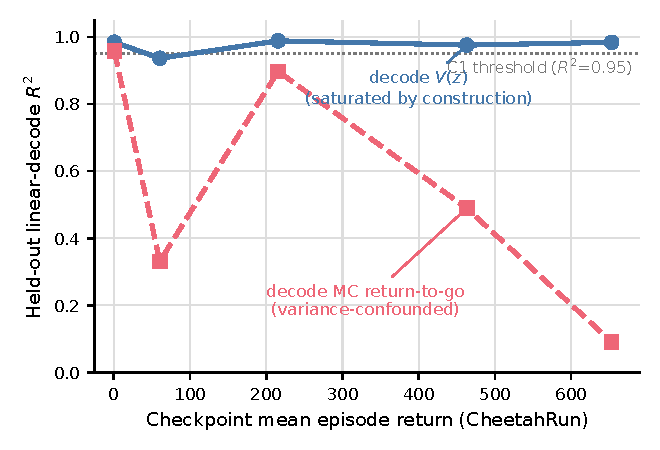
\includegraphics[width=0.62\linewidth]{figures/fig_r2_discrimination.pdf}
\caption{\textbf{The value-decodability probe does not discriminate.} Held-out, ridge-regularized linear-decode $R^2$ against checkpoint quality, across five CheetahRun checkpoints spanning the full performance range --- from a collapsed policy (return $0.8$) to a strong one (return $653$), including distractor-augmented variants (0--128 injected distractor dimensions); $n{=}6{,}000$ held-out states (6 episodes) per checkpoint, single seed. Decoding the value network's own output $V(z)$ (blue, circles) is saturated by construction ($R^2 \geq 0.94$ everywhere, above the criterion's 0.95 threshold at both extremes of policy quality); decoding the Monte-Carlo return-to-go (red, squares) is dominated by return variance --- highest ($0.96$) for the collapsed policy, lowest ($0.09$) for the strong one, and non-monotone in between. Neither operationalization varies with the quantity C1 claims to measure. Data: \texttt{evidence/vzprobe/*.json}.}
\label{fig:r2disc}
\end{figure}

\paragraph{Disproof of C1 as an operational criterion (2026-06).} The reading above is seductive but \emph{wrong as a criterion}: a high linear-decode $R^2$ does not certify value-sufficiency, because it does not \emph{discriminate}. We ran a held-out, ridge-regularized discrimination experiment that probes the same latent two ways across CheetahRun checkpoints spanning the full performance range (return $1$ = collapsed policy $\to$ $653$ = strong); Figure~\ref{fig:r2disc} shows the result. Decoding the value network $V(z)$ gives $R^2\approx0.98$ \emph{flat} --- $0.984$ at return $653$, $0.984$ at return $1$, unchanged by up to $128$ injected distractor dimensions --- because $V$ is computed by a near-linear head on $z$, so $V$ is \emph{always} linearly recoverable regardless of policy quality or representation. The $R^2{=}0.9994$ above is this same artifact. Decoding the Monte-Carlo return-to-go instead anti-tracks performance through a variance confound (a collapsed policy has near-constant returns, trivially ``decodable'': $R^2{=}0.96$ at return $1$ vs.\ $0.09$ at return $653$). Neither operationalization of C1 measures value-sufficiency in a way that varies with the quantity it claims to measure. We could not even \emph{construct} a low-$R^2$ regime: distractors did not lower $V(z)$-decodability. C1 is therefore \textbf{not} a usable predictive criterion. What survives is the empirical fact --- every value-organizing objective on this latent was null --- with C1 demoted from ``criterion'' to ``failed instrument,'' and the methodological lesson that a mechanism metric must be shown to discriminate before it is trusted.\footnote{Evidence files: \texttt{evidence/vzprobe/*.json} (V(z) vs.\ return-to-go held-out $R^2$ across the performance range); discrimination-matrix details in the project's Part-13 report.}

\textbf{C2 --- pre-existing interaction structure (holds for (a), fails for (b)).} The SimNorm latent's \emph{transition graph} already carries strong community structure. On a trained jumpy CheetahRun checkpoint, dumping 12{,}000 latents, clustering to 128 nodes, and building the $k$-step transition graph, the SE-optimal partition yields a best compression gap of \textbf{53.1\%} (and \textbf{47.2\%} for a kNN-on-centroids graph).\footnote{Evidence file: \texttt{evidence/se\_precheck\_simnorm\_cheetah.json} in the paper repository --- persisted re-run of the tier-2 analysis (\texttt{scripts/persist\_se\_precheck.py}) on the original latent dump, reproducing the figures first recorded in the source repository's \texttt{docs/research/se-precheck-note.md} \S6.} Crucially this was measured on a \emph{jumpy encoder trained with no SE pressure}, ruling out the objection that the structure is an artifact of a clustering loss. So C2(a) --- the structure is already present --- holds, and an SE-clustering objective can only re-derive it.

But C2(b) fails: the communities are \textbf{motion phases} (swing / stance / contact arcs of the limit cycle), not control-relevant subgoals or error-prone regions.\footnote{Source repository: \texttt{docs/analysis/why-glass-failed-simnorm-redundancy.md} \S3; \texttt{docs/research/se-precheck-note.md} \S2.} An SE objective that imposes this structure trades control-relevant capacity for structure the model did not need --- which is the misaligned-structure failure mode. The early Glass clustering levers (geometric and behavioral prototype clustering) were null at adequate sample size for exactly this reason.\footnote{Source repository: \texttt{docs/iterations/RESEARCH\_LEDGER.md}, nulls \#1--\#2.}

Summary for the monolithic class: C2 is measured directly (structure present but control-irrelevant), and every clustering / value-equivalence lever was null or harmful. C1's apparent satisfaction, by contrast, is an instrument artifact and contributes no evidence. The redundancy conclusion for this class therefore rests on the direct experimental record --- the campaign's nulls (Section~\ref{sec:campaign}) and the matched 16-task benchmark that follows (Section~\ref{sec:benchmark}) --- not on the probe.

% ============================================================================
% DRAFT replacement/augmentation for main.tex section 4.1 "Monolithic (TD-MPC2/SimNorm)".
% Status: for review, NOT yet spliced. Numbers from evidence/dmc_glass_vs_tdmpc2.json (n=3
% both algos; seed-4 in flight will tighten CIs further -> live page authoritative).
% NOTE: this version corrects an n=2 over-read: at n=3 there is NO systematic return
% difference and NO systematic stability difference (both algos have collapsing seeds);
% the only robust effect is the 1.35x wall-clock cost. That is the strongest null.
% ============================================================================

\subsection{Monolithic (TD-MPC2 / SimNorm): a matched, multi-seed benchmark}
\label{sec:benchmark}

The strongest single piece of evidence for representation-abstraction redundancy is a
matched-protocol benchmark of the explicit structural-entropy (SE) abstraction
(\emph{tdmpc-glass}) against the identical monolith (\emph{tdmpc2}) --- same code,
hyperparameters, and harness, the SE objective the only changed variable --- across
\textbf{16 DMControl tasks at 1M environment steps}, with \textbf{mean $\pm$ 95\% CI over $n{=}4$
seeds} and a \textbf{wall-clock} axis (Table~\ref{tab:bench}). This upgrades the single-run levers
of \S\ref{sec:campaign} to a controlled multi-seed comparison.

\begin{table}[t]
\centering\small
\caption{DMControl return at 1M steps, tdmpc-glass (SE abstraction) vs.\ tdmpc2 (monolith),
mean$\pm$95\%CI ($n{=}4$), and per-run wall-clock. No systematic return difference (ties within CI
on 15/16; the single CI-separated case favors the monolith and tracks a collapsed glass seed); the only
robust effect is $\sim$1.35$\times$ wall-clock. Source: \texttt{evidence/dmc\_glass\_vs\_tdmpc2.json}.}
\label{tab:bench}
\begin{tabular}{lrrl}
\toprule
task & tdmpc-glass & tdmpc2 & note \\
\midrule
WalkerWalk      & $919{\pm}80$  & $971{\pm}12$  & tie \\
WalkerStand     & $969{\pm}14$  & $979{\pm}16$  & tie \\
WalkerRun       & $662{\pm}8$   & $652{\pm}34$  & tie \\
CartpoleBalance & $972{\pm}9$   & $945{\pm}50$  & tie \\
CartpoleSwingup & $836{\pm}12$  & $823{\pm}35$  & tie \\
FingerSpin      & $969{\pm}12$  & $950{\pm}32$  & tie \\
FingerTurnEasy  & $874{\pm}96$  & $920{\pm}84$  & tie \\
FingerTurnHard  & $725{\pm}155$ & $869{\pm}167$ & tie (both noisy) \\
AcrobotSwingup  & $296{\pm}11$  & $324{\pm}99$  & tie \\
HopperHop       & $196{\pm}142$ & $265{\pm}63$  & tie (both noisy) \\
BallInCup       & $486{\pm}477$ & $731{\pm}414$ & tie (both noisy) \\
ReacherEasy     & $933{\pm}87$  & $980{\pm}3$   & tie/glass-noisy \\
CheetahRun      & $658{\pm}7$   & $500{\pm}268$ & tie (tdmpc2 noisy) \\
ReacherHard     & $976{\pm}2$   & $883{\pm}148$ & tie (tdmpc2 noisy) \\
HopperStand     & $417{\pm}323$ & $896{\pm}35$  & tdmpc2$>$ (glass bad seed) \\
PendulumSwingup & $389{\pm}382$ & $589{\pm}336$ & tie (both noisy) \\
\midrule
\textbf{wall-clock (mean, min/run)} & \textbf{80.6} & \textbf{59.8} & \textbf{1.35$\times$} \\
\bottomrule
\end{tabular}
\end{table}

\begin{figure}[t]
\centering
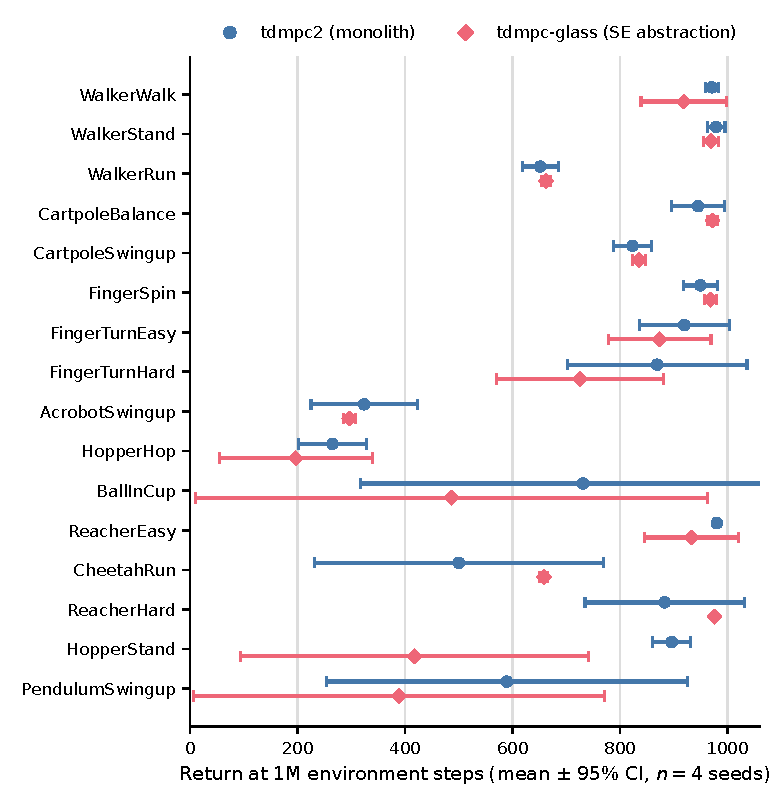
\includegraphics[width=0.72\linewidth]{figures/fig_benchmark_forest.pdf}
\caption{\textbf{Forest plot of the matched 16-task DMC benchmark} (the data of
Table~\ref{tab:bench}): return at 1M environment steps, mean $\pm$ 95\% CI over
$n{=}4$ seeds per arm, tdmpc2 monolith (blue circles) vs.\ tdmpc-glass SE abstraction
(red diamonds), identical code/hyperparameters/harness with the SE objective the only
changed variable. CIs overlap on 15/16 tasks; the single separated case (HopperStand)
favors the monolith and tracks one collapsed glass seed. The SE abstraction buys no
systematic return difference while costing $\sim$1.35$\times$ wall-clock.
Data: \texttt{evidence/dmc\_glass\_vs\_tdmpc2.json}.}
\label{fig:benchforest}
\end{figure}

\paragraph{Findings.}
(1) \emph{No systematic return effect} (Figure~\ref{fig:benchforest}). On 15 of 16 tasks the two tie within overlapping
95\% CIs; the single CI-separated case (HopperStand) favors the monolith and is attributable to a
\emph{single collapsed glass seed}, not a consistent capability gap. The SE objective
produces no systematic gain (nor, at $n{=}4$, a systematic loss). (2) \emph{No systematic stability
difference either.} Both algorithms exhibit occasional seed collapses at this scale (tdmpc2 noisy on
CheetahRun/ReacherHard/BallInCup, glass on HopperStand/Pendulum), so an apparent ``glass is less stable''
read at low $n$ does not survive; the honest statement is high-variance-both-sides at low
seed count. (3) \emph{The one robust difference is cost:} the SE objective adds $\sim$35\%
wall-clock per matched-budget run. The verdict for the monolithic class is therefore the
strongest form of redundancy: \textbf{explicit SE abstraction changes return by nothing detectable
at $n{=}4$ while costing 1.35$\times$ the compute} --- the empirical fingerprint of a basis change
that relocates rather than removes complexity (\S\ref{sec:mechanism}).

\paragraph{A methodological note (why multi-seed was necessary, in both directions).}
A single-seed read of this benchmark would have been misleading \emph{twice over}. On the
high-variance tasks (HopperHop, BallInCup, PendulumSwingup, HopperStand) a single glass run can
look like a ``catastrophic failure'' that the seed spread refutes --- e.g.\ glass HopperHop is
$196{\pm}142$ ($n{=}4$), a variance band, not a capability gap. Symmetrically, at low seed count
tdmpc2 looked uniformly tight and glass uniformly noisy, inviting a ``glass is unstable'' claim that
more seeds refuted (tdmpc2 collapses too --- it is the noisy side on CheetahRun/ReacherHard/BallInCup).
Extreme single measurements invite over-claims in \emph{both}
directions; CI-over-seeds is what separates a result from an artifact --- the same lesson as the
value-decode probe of \S\ref{sec:criterion}, where a single saturated $R^2$ masqueraded as proof.


\subsection{Token-transformer (attention graph): a measured NO-GO}
\label{sec:transformer}

For a token-transformer WM the natural interaction graph is the attention graph. We trained a transformer-WM on PandaPickCube and ran \texttt{scripts/se\_attention\_graph.py}, which rolls out the actor, aggregates per-layer attention into a $(T \times T)$ adjacency ($T=32$ tokens, 4 layers, 4 heads), sparsifies (quantile thresholds and kNN), and compares the SE compression gap against a \emph{degree-preserving null} that destroys community structure while preserving the weight distribution. Only the margin over this null counts as real structure; raw gaps are inflated by sparsification.

The verdict is \textbf{NO-GO}. The best per-layer compression gap \emph{over the null} is $\mathbf{-0.0334}$ for the trained model (best layer 0) and $\mathbf{+0.0064}$ for an architecture-matched untrained model (best layer 1).\footnote{Evidence files: \texttt{evidence/se\_attn\_trained.json}, \texttt{evidence/se\_attn\_untrained.json} in the paper repository.} Both are below the GO margin threshold of 0.05, so neither model has exploitable community structure; the per-layer over-null margins for the trained model are $-0.0334$ (L0), $-0.1217$ (L1, knn4), $-0.0987$ (L2, knn4), $-0.0307$ (L3) at their best variants.\footnote{Evidence file: \texttt{evidence/se\_attn\_trained.json} in the paper repository.} The decisive comparison is trained $\approx$ untrained: training induces \textbf{no} exploitable community structure in the attention graph. This is the C2 ``no structure'' failure mode (as opposed to the monolithic class's ``wrong structure''). An SE-as-a-loss has nothing to shape on this substrate, and the cheap probe killed the SE-loss build before it was written.\footnote{Source repository: \texttt{docs/iterations/iteration\_28\_plan.md}, ``NORTH-STAR SE-ATTENTION-GRAPH VERDICT''.}

\textbf{Scope (honest).} This is the \emph{attention} graph of a small, modestly-trained transformer-WM ($\sim$16k training steps; checkpoint eval $\sim$345) on \emph{single-object} manipulation, where relational structure is inherently weak.\footnote{Evidence file: \texttt{evidence/se\_attn\_trained.json} (meta block) in the paper repository; source repository: \texttt{docs/iterations/iteration\_28\_plan.md}.} It does \textbf{not} close the case for a true entity-node graph/GNN WM on a genuinely relational (multi-object / multi-agent) domain. The attention-graph \emph{proxy} for graph-WM+SE is dead; the entity-graph version is the remaining open class (Section~\ref{sec:entitygraph}).

\subsection{Entity-graph latents: a synthetic instrument-validation NO-GO}
\label{sec:entitygraph}

The entity-graph class is the one where the criterion's positive direction is most plausible, and it makes a clear \emph{prediction} together with a pre-specified mechanism-check: train an entity-factored WM, probe (i) C1 via \texttt{value\_probe} --- is value linearly decodable from the flat entity concatenation, and critically does $R^2$ \emph{drop} at held-out object counts? --- and (ii) C2 via an SE-gap computation on the \emph{value-coupling} interaction graph (edge weight $=$ sensitivity of return to an entity-pair interaction), not the similarity graph.\footnote{Source repository: \texttt{docs/research/graph-wm-se-proposal.md} \S A; \texttt{docs/research/graph-wm-dr/dr1-fable5-graph-wm-se-survey.md} \S``Cheap mechanism-check''.} The criterion predicts redundancy (a null) \textbf{unless} C1 fails OOD --- i.e.\ value stops being linearly decodable at held-out object counts --- in which case the entity-graph class would be the first to exhibit genuine headroom for explicit abstraction. (This was the pre-specified plan; note that after the disproof of Section~\ref{sec:monolithic}, running it requires a decodability instrument that first passes an in-distribution discrimination test, which the naive linear probe does not.)

Before any real multi-object build, we validated the prescribed \emph{instrument} on a controlled synthetic gate, and the result is the third measured data point --- a NO-GO. We built a synthetic multi-entity world whose ground-truth value coupling is \emph{known by construction}: the reward is $-\lVert p_0 - p_1 \rVert - w \lVert p_2 - p_3 \rVert$, so value couples \emph{only} the entity pairs $\{(0,1), (2,3)\}$. We trained a flat entity-transformer WM on it and probed whether a \textbf{value-coupling graph} ($w_{ij} = \mathbb{E}\,\lVert \partial^2 r / \partial s_i\, \partial s_j \rVert_F$, the input cross-Hessian; also a $Q$-head variant) recovers the known pairs, against a label-shuffle null and against similarity and attention graphs.\footnote{Evidence file: \texttt{evidence/gate0b\_vcoupling.json} in the paper repository (probe: \texttt{scripts/value\_coupling\_probe.py}; environment: \texttt{src/helios/envs/synthetic\_entities.py}; WM: \texttt{entity\_wm.py} in the source repository).}

The verdict is \textbf{NO-GO in-distribution, with a near-perfect reward fit} (reward loss $0.0026$): the value-coupling graph scores AP $=\mathbf{0.500}$ at $z=\mathbf{-0.08}$ over the label-shuffle null --- i.e.\ at chance relative to the null (chance AP $=0.33$); the $Q$-head variant is identical; and the \textbf{similarity graph (AP $=\mathbf{0.750}$, $z=1.38$) and attention graph (AP $=0.750$, $z=1.42$) beat it} (value$-$similarity AP $= -0.25$). Even the winners are not significant ($z<3$; only 6 candidate pairs at $N=4$ entities).\footnote{Evidence file: \texttt{evidence/gate0b\_vcoupling.json} in the paper repository.} The mechanism: the transformer computes the correct reward but routes the dependence through attention-mixing and mean-pooling, so the input cross-Hessian reflects \emph{computational mixing}, not \emph{semantic coupling}. This is in one sense the cleanest of the three data points: the coupling structure provably \emph{exists} in the environment, yet the instrument cannot expose it from the trained WM.

\textbf{Caveats (honest).} (a)~This tests the \emph{input cross-Hessian} operationalization of value coupling; the proposal's literal form was message-level ($\lvert \partial Q / \partial \text{message}_{ij} \rvert$). The closest proxy tested (the attention graph) is also non-significant, but a true attention-\emph{edge ablation} (zero out edge $i$--$j$, measure $\Delta$reward) requires model surgery and is \textbf{untested}. (b)~The OOD-by-distractor variant of the gate is confounded (the reward depends on fixed entity indices, so the model needs identity embeddings and held-out slots carry untrained embeddings); only the in-distribution result is confound-free. (c)~The result is synthetic, on a small WM, at a single seed. The full-scale prediction of Section~\ref{sec:predictions} --- abstraction helps iff C1 collapses OOD on a real multi-object task --- therefore remains open; what is measured here is that the value-coupling instrument, as operationalized, reads at chance even when ground-truth coupling structure is present.

\paragraph{Hardened OOD decodability sweep (measured, synthetic world, $n{=}4$).} After the instrument disproof of Section~\ref{sec:monolithic}, we still ran the pre-specified OOD decodability sweep at scale in the synthetic entity world --- trained at $N{=}4$ objects, probed at held-out $N' \in \{6,8,10,12,14\}$ (up to $3.5\times$ the training count), $n{=}4$ seeds, held-out ridge decode of Monte-Carlo return-to-go --- reading it \emph{comparatively across architectures}, not as a certification (the instrument caveats above apply).\footnote{Evidence files: \texttt{evidence/entity\_graph\_go\_hardened/seed\{0..3\}.json} in the paper repository.} Two readings. (i)~\emph{Re-fit} decodability (probe re-fit at each $N'$) shows \textbf{no OOD cliff for any architecture}: the monolith holds $0.75$--$0.86$ across the sweep ($0.857 \pm 0.014$ at $N'{=}14$) and the entity-factored WM $0.79$--$0.87$ ($0.867 \pm 0.013$ at $N'{=}14$) --- the entity-graph latent gains \emph{no} decodability headroom out-of-distribution, which is the ``no collapse $\Rightarrow$ abstraction stays redundant'' branch of Section~\ref{sec:predictions} and extends the earlier NO-GO out to $N'{=}14$. (ii)~The \emph{frozen-probe transfer} view (probe fit at $N{=}4$, applied unchanged) does separate architectures: the entity latent retains weakly positive transfer ($0.47 \pm 0.19$ at $N'{=}10$; $0.26 \pm 0.36$ at $N'{=}14$) while the zero-padded monolith collapses catastrophically ($-10.0 \pm 7.0$ at $N'{=}14$) --- a genuine representation-\emph{stability} difference that nonetheless converts into no re-fit capacity advantage. Scope: synthetic world, uncertified linear instrument; comparative evidence only, and the real-task OOD cell stays open.

\section{The 16-null campaign as systematic evidence}
\label{sec:campaign}

The criterion did not come from a single experiment; it is the compression of a campaign of explicit-abstraction levers, each run under a single-variable, compute-matched protocol with pre-registered peak-and-final CI gates \citep{agarwal2021rliable} and a mechanism-check before any multi-seed fan-out.\footnote{Source repository: \texttt{docs/iterations/RESEARCH\_LEDGER.md}, ``Gate discipline''.} Table~\ref{tab:nulls} summarizes the levers and why each died; all entries are read from the ledger.

\begin{table}[t]
\centering
\caption{The explicit-abstraction lever campaign: every lever was null or harmful. All rows are read from the source repository's research ledger (\texttt{docs/iterations/RESEARCH\_LEDGER.md}, ``WHAT DID NOT WORK'') and \texttt{docs/iterations/iteration\_28\_plan.md} (``ARCH A/B VERDICT'') for \#15. Evidence file for row 1: \texttt{evidence/clustering\_panda\_pick\_n5.json}.}
\label{tab:nulls}
\footnotesize
\begin{tabular}{@{}r p{3.6cm} l p{6.6cm}@{}}
\toprule
\# & Lever & Outcome & Why (per ledger) \\
\midrule
1 & Geometric prototype clustering (SE Glass) & NULL & redundant with SimNorm's soft-categorical latent (IQM 0.748 vs 0.738, overlapping); confirmed on manipulation at $n{=}5$ (PandaPickCube final 1247 CI~[815, 1693] $\approx$ vanilla 1416 CI~[1010, 1821]) \\
2 & Behavioral / reward-grounded clustering & NULL & null at $n{=}34$; gain crossed CI-separation then settled in overlap \\
3 & Bisimulation auxiliary \citep[BS-MPC style;][]{shimizu2025bsmpc} & HARMFUL & actively hurts (0.549); brittle to coefficient; failed twice \\
4 & Distractor robustness from abstraction & FALSIFIED & $1.23\times < 1.5\times$ gate; both encoders crushed equally \\
5 & Sparse-task rescue via grouping & NULL & exploration problem, not latent geometry (0/3 vs 1/3) \\
6 & ``Floor effect'' / weak-seed tail & INVERTED & behavioral arm produced the worst seed (0.127) \\
7 & Laplacian / eigenpurpose exploration & NULL & generic RND $\geq$ it everywhere \\
8 & Community-detection skills & NULL & communities = motion phases, not reachable subgoals \\
9 & $\rho$ consistency-horizon schedule & NULL & task-dependent tuning knob, not architecture \\
10 & SE-$k$ adaptive jump-length & NULL & SE pre-check passed (53\% gap) but boundary score does not track $k$-step error (Spearman $+0.09$ / $-0.18$) \\
11 & Uncertainty-gated horizon (F) & NULL & signal valid (Spearman 0.72) but no headroom; $k$-step error uniform in-dist (inflation $1.06\times$) \\
12 & SI2E / VCSE SE-exploration & NULL & no rescue of sparse tasks; does not beat RND; at coef 1.0 mildly hurts \\
13 & wmsi2e --- SE-exploration over WM latent & NULL & ties SI2E at 0/$n$; adds nothing over random-encoder SI2E or RND \\
14 & Value-equivalence loss & NULL & coef sweep monotone harm; no coefficient beat baseline on peak and final (\S\ref{sec:monolithic}; the supporting $R^2$ probe reading was later retracted as saturated) \\
15 & Alt dynamics backbone (resmlp / attn) & NULL/mirage & helps weak vanilla ($+40\%$/$+26\%$) but hurts strong jumpy (jum/resmlp 1796/1381 $\ll$ jum/mlp 2645/2319) \\
\bottomrule
\end{tabular}
\end{table}

Two cross-cutting findings recur. First, the \textbf{uniform-error} finding: a strong jumpy model is uniformly accurate over the states a near-optimal policy visits, which is why fixed-$k$ jumpy works and why every \emph{adaptive} scheme (\#10, \#11) has nothing to adapt to.\footnote{Source repository: \texttt{docs/iterations/RESEARCH\_LEDGER.md}, ``Root cause for \#10--11''.} Second, the \textbf{redundancy} finding: a strong self-predictive WM (TD-MPC2 + SimNorm) already encodes a value-sufficient abstraction, so explicit clustering / value objectives re-derive structure already present.\footnote{Source repository: \texttt{docs/iterations/RESEARCH\_LEDGER.md}, ``Cross-cutting lesson''.} The criterion makes the second finding measurable and predictive.

\textbf{The campaign's one positive result is consistent with the criterion --- and narrower than our interim notes claimed.} The only lever that beat the baseline was the (prior-art) jumpy / $k$-step world model itself \citep{farebrother2026jumpy} --- \emph{not} an abstraction objective. The picture is task-dependent rather than suite-wide (persisted aggregations, 10k-resample bootstrap on seed means): PandaPickCubeOrientation is a clean CI-separated win at $n{=}5$ per arm (jumpy final 2145 vs vanilla 1129, $+90\%$, difference CI95 [685, 1344]; every jumpy seed beats every vanilla seed); PandaPickCube, a positive trend that had not reached CI separation at $n{=}5$ (1872 vs 1416, $+32\%$, difference CI95 [$-267$, 1169]), \emph{resolved} once boosted to $n{=}8$ per arm: jumpy 1969 vs vanilla 1355, $+45\%$, difference CI95 [66, 1153] --- now CI-separated; PandaOpenCabinet is null at $n{=}5$ (1050 vs 1053, difference CI95 [$-563$, 685]).\footnote{Evidence files: \texttt{evidence/anchor\_jumpy\_vs\_vanilla.json} (the $n{=}5$ aggregation, from \texttt{scripts/aggregate\_anchor.py}) and \texttt{evidence/p1\_score.json} (\texttt{pick\_anchor\_n8} block) with per-seed finals in \texttt{evidence/p1\_ksweep\_harvest.json}, in the paper repository.} Jumpy's scoreboard is thus 2/3 tasks CI-separated (PickCube, Orientation) plus one null (OpenCabinet). Earlier hand-aggregated interim numbers ($+101\%$/$+75\%$/$+74\%$ across all three tasks at $n{=}2$--$4$) settled as seeds completed --- itself a demonstration of why we persist aggregations and report final-$n$ CIs. Peak is mixed (vanilla often higher peak; jumpy sustains final where it wins). Jumpy is a temporal, not an abstraction, lever --- consistent with the thesis that abstraction is the redundant axis on this substrate while temporal coarse-graining (on some tasks) is not. Section~\ref{sec:scored} turns this task-dependence itself into a scored, pre-registered prediction.

% ============================================================================
% DRAFT section for wm-redundancy-paper — Theory/Mechanism + Scope.
% Status: for review, NOT yet spliced into main.tex.
% Purpose: supply the MECHANISM the current draft lacks (it measures the null
% but does not explain it), in a way CONSISTENT with the dead R^2 probe.
% ============================================================================

\section{Why redundancy holds: abstraction is a basis change, not a capacity change}
\label{sec:mechanism}

The campaign establishes \emph{that} explicit representation abstraction is null on
TD-MPC2/SimNorm; this section argues \emph{why}, and reconciles the mechanism with our
negative methodological result that a linear value-decode $R^2$ cannot certify it
(\S\ref{sec:criterion}).

\paragraph{Abstraction redistributes complexity; it does not remove it.}
An explicit abstraction $\psi$ added to a world model does not enlarge the realizable
hypothesis class: a monolithic latent and an explicitly factored one can represent the same
value function. What $\psi$ changes is the \emph{basis} in which control is expressed --- the
analogue of \emph{separation of concerns} in software engineering, which never reduces a
program's intrinsic complexity but reshapes where it lives to lower a bounded agent's
search-and-maintenance cost. Writing a task's difficulty heuristically as
$\mathcal{C}_{\text{task}} \approx \mathcal{C}_{\text{represent}} + \mathcal{C}_{\text{control}}$,
an abstraction moves mass from $\mathcal{C}_{\text{control}}$ (a policy over a tidy abstract
space) into $\mathcal{C}_{\text{represent}}$ (building and keeping the abstraction correct).
It is a change of basis on a conserved total. It can only help a learner if the new basis is
\emph{better conditioned for that learner on that task} --- i.e.\ if it lowers \emph{statistical
or optimization} cost, never the information content.

\paragraph{The capacity channel is closed by sufficiency (data processing).}
TD-MPC2's SimNorm latent $\phi$ is trained, by its self-predictive, reward, and TD objectives,
to be a sufficient statistic for value and dynamics: when this succeeds, $Q^\star(s,a)$ is
measurable with respect to $\phi(s)$. Any explicit abstraction $\psi$ is a deterministic
function of the state; if it factors through an already value-sufficient $\phi$, the
\emph{data-processing inequality} forbids it from adding task-relevant information.

\begin{proposition}[Capacity-channel redundancy, informal]
\label{prop:dpi}
If $\phi$ is value-sufficient ($Q^\star$ is $\sigma(\phi)$-measurable), then for any
deterministic abstraction $\psi$, post-composing or adjoining $\psi$ cannot raise the realizable
optimum. Hence any effect of explicit abstraction must act through the \emph{optimization /
sample-complexity} channel, not the representational-capacity channel.
\end{proposition}

The reason the monolith reaches this regime \emph{without} an explicit module is the
value-equivalence principle \citep{grimm2020value}: a model need only be correct for value and
planning, not for full reconstruction, and end-to-end self-prediction on a single task already
finds that value-equivalent (implicitly bisimulation-like; \citealp{ferns2004,castro2020,gelada2019})
abstraction. The monolith \emph{implicitly modularizes}; an explicit module is then redundant ---
the concern it would separate is already separated inside $\phi$.

\paragraph{Reconciliation with the failed probe.}
Proposition~\ref{prop:dpi} and our $R^2$ negative are complementary, not contradictory. The
proposition explains the empirical null: the latent \emph{is} sufficient, so abstraction buys
nothing on return. The methodological result (\S\ref{sec:criterion}) shows only that a
\emph{linear decode} cannot \emph{certify} this sufficiency --- $V(z)$-decode is saturated by
construction and return-to-go decode is variance-confounded. The honest joint statement is
therefore: \emph{the latent is value-sufficient enough that explicit abstraction is redundant,
but linear decodability is not a valid certificate of that sufficiency.} A valid certificate
would need a decode whose accuracy is invariant to policy quality and not realized by the value
head's own near-linearity --- which our experiments show the obvious probes are not.

\paragraph{The cost axis is the empirical fingerprint of ``redistribute, not reduce.''}
The basis-change account makes a prediction the pure-return null does not: an explicit
abstraction should add representation-upkeep cost for no capacity gain. The matched DMC
benchmark (\S\ref{sec:benchmark}) confirms it --- the structural-entropy abstraction
(tdmpc-glass) matches the monolith on return within confidence intervals (no systematic
difference either way at $n{=}4$) while costing $\sim$35\% more wall-clock per matched-budget run
($1.35\times$). The conserved complexity was relocated into the abstraction, not removed.

\paragraph{Caveat on the conservation heuristic.}
$\mathcal{C}_{\text{task}}=\mathcal{C}_{\text{represent}}+\mathcal{C}_{\text{control}}$ is an
intuition pump, not a proven identity; the rigorous core is Proposition~\ref{prop:dpi}
(information cannot be created by post-processing) and the value-equivalence reduction. A formal
version would decompose sample complexity into a representation-learning and a
policy-optimization term and show the basis change trades between them.

\section{Scope: when explicit/structured abstraction is \emph{not} redundant}
\label{sec:scope}

The redundancy claim is bounded, and the boundary follows from the mechanism:
explicit abstraction is redundant exactly when end-to-end optimization is \emph{not} the
bottleneck (the monolith already finds the value-sufficient latent). It stops being redundant
when the optimization/sample channel binds --- and there the gain is on axes other than asymptotic
return. Two regimes lie outside this paper's negative claim and are reported separately
(companion work): (i) \emph{behavioral} priors in the action loop (an analytic controller with a
learned residual, or a structured-skill-to-free-policy curriculum) beat a strong model-free
baseline on \emph{sample-efficiency and stability} on exploration-/credit-assignment-limited
manipulation tasks, where the naive learner is optimization-limited; and (ii) the same recipe
\emph{backfires} when the injected prior is wrong (a weak controller on an underactuated
swing-up becomes an anchor the policy must fight). A budget-matched control sharpens (i): on
dense-reward continuous-control tasks that a strong baseline already solves at the matched step
budget (a swept set of DMControl locomotion and reaching tasks), an analytic-controller-plus-residual
yields \emph{no asymptotic gain} over a matched-budget model-free baseline --- it ties or loses on
final return --- and its only robust advantage is sample-efficiency, and only when the prior captures
the task's control-relevant substructure (the actuated degrees of freedom coincide with the goal
degrees of freedom). The apparent ``beats the baseline'' wins in our interim notes were against an
\emph{under-budgeted} baseline; against a step-matched one they reduce to a head-start, not a higher
ceiling. This is itself a behavioral echo of the representational redundancy result: extra structure
buys conditioning, not capacity. Both are consistent with the present account:
abstraction helps only when it supplies structure the monolith genuinely lacks, and a value-
sufficient single-task latent lacks none. This is the constructive complement to the negative
campaign, and it scopes the redundancy result to \emph{representation} abstraction on a value-
sufficient latent rather than to abstraction in general.


\section{Predictions \& falsification}
\label{sec:predictions}

The criterion is useful only if it makes risky predictions. It does:

\begin{enumerate}
\item \textbf{A positive case requires C1 to fail.} Explicit abstraction will help control only on a latent where value is \emph{not} linearly decodable on the relevant distribution. The sharpest place to test this is the compositional / OOD regime: train an entity-factored WM on $N$ objects and probe value-decodability at held-out $N' \neq N$. The criterion predicts a control gain from abstraction \textbf{iff} decodability \emph{collapses} OOD; if it stays high OOD, abstraction stays redundant.\footnote{Source repository: \texttt{docs/research/graph-wm-se-proposal.md} \S B-3, \S``GO only if\ldots''.} Any such test must first fix the instrument: the naive linear decode fails the in-distribution discrimination test of Section~\ref{sec:monolithic}, so a collapse (or its absence) measured with it would be uninterpretable.

\item \textbf{No-structure vs wrong-structure are distinguishable a priori.} C2 splits into ``gap at/below null'' (token-transformer attention, Section~\ref{sec:transformer}) and ``gap above null but task-misaligned'' (SimNorm motion phases, Section~\ref{sec:monolithic}). The criterion predicts an SE objective is unhelpful in \emph{both} cases, and the SE-gap-vs-null + alignment probes diagnose which one applies before any build.

\item \textbf{Value-coupling beats similarity.} If an entity-graph latent satisfies C1 OOD-collapse, the criterion predicts the \emph{value-coupling} graph (edges $= \partial\,\text{return}/\partial\,\text{interaction}$), not the similarity graph, is the one that carries task-aligned structure --- because the sparse relational structure of \emph{which interactions drive return} is a property of the dynamics graph that a monolithic latent does not expose.\footnote{Source repository: \texttt{docs/research/graph-wm-se-proposal.md} \S B-1.} A positive counterexample here would both falsify the ``abstraction is always redundant'' reading and confirm the criterion's predictive direction. The synthetic gate of Section~\ref{sec:entitygraph} already cuts against the \emph{input cross-Hessian} operationalization of this prediction --- there, similarity beat value-coupling even though ground-truth coupling existed --- so a positive test of this prediction must first fix the instrument (e.g.\ attention-edge ablation).
\end{enumerate}

A clean falsification of the redundancy claim itself would be: a trained latent on a substrate like ours (self-predictive, value-sufficient by the direct behavioral test) for which a single-variable explicit-abstraction objective nonetheless produces a $\geq 10\%$, CI-separated control gain on $\geq 3/4$ tasks under the campaign's protocol. We did not observe one in 16 levers. (We deliberately no longer state this falsification test in terms of an $R^2 \gtrsim 0.95$ precondition: Section~\ref{sec:monolithic} shows the linear probe cannot certify that precondition.)

\subsection{A scored, pre-registered positive direction}
\label{sec:scored}

The redundancy criterion says where abstraction is redundant. The converse question --- where does \emph{temporal} abstraction pay? --- we made predictive, and then scored. The campaign's one positive lever (the jumpy $k$-step model) has task-dependent gains (Section~\ref{sec:campaign}), which raises a testable question: is there a checkpoint-computable signal that predicts, per task, how much jumpy will gain? We screened nine candidate signals (error medians and dispersions, latent speeds, disagreement statistics, perturbation inflation), computed from a single trained $k{=}4$ checkpoint per task, against the measured jumpy final-return gains at the time of the screen ($+90\%$ Orientation / $+32\%$ PickCube / $0\%$ OpenCabinet). Exactly one survived the ordering screen:
\[
\texttt{disc\_err\_gap} \;=\; \frac{\mathrm{median}(\text{disagreement})}{\mathrm{median}(\text{true $k$-step error})}
\qquad \text{Ori } 1.33 \;>\; \text{Pick } 1.12 \;>\; \text{Cab } 0.95,
\]
where \emph{disagreement} is the ensemble-free jumpy-vs-iterated-one-step prediction gap --- computable from one checkpoint, no ground truth needed.\footnote{Evidence file: \texttt{evidence/p1\_temporal\_signals.json} in the paper repository (9 candidates, \texttt{surviving\_candidates} = [\texttt{disc\_err\_gap}]).} The reading: temporal abstraction pays where the macro-model is accurate \emph{and} calibrated-conservative (disagreement $\geq$ error); it fails where the model is inaccurate and overconfident. An ordering match at $n{=}3$ tasks is hypothesis-generating only, so we pre-registered the test: fresh jumpy variants at $k{=}2$ and $k{=}8$ (effective planning horizon fixed, compute-matched) were trained on all three tasks, the signal was computed from their dumped checkpoints, and the predictions were committed to a public git history \textbf{before any final return was read} ($k{=}2$ gaps 0.969/1.028/0.672 all below their $k{=}4$ values $\Rightarrow$ predict lower gains at $k{=}2$; $k{=}8$ gaps 1.521/1.736/1.681 all above $\Rightarrow$ predict higher gains at $k{=}8$).\footnote{Evidence file: \texttt{evidence/p1\_ksweep\_prediction.json} in the paper repository; the source repository's git history timestamps the commit order.} Table~\ref{tab:scored} shows the score against finals read for the first time at harvest.

\begin{table}[t]
\centering
\caption{Scored pre-registered predictions ($k$-sweep, final returns, $n{=}3$ seeds per new cell). All rows read from \texttt{evidence/p1\_score.json} and \texttt{evidence/p1\_ksweep\_harvest.json}.}
\label{tab:scored}
\footnotesize
\begin{tabular}{@{}llll@{}}
\toprule
Block & Prediction & Outcome & Scored \\
\midrule
Pick $k2{<}k4$ & lower gain at $k{=}2$ & 1616 vs 1969 & \checkmark \\
Ori $k2{<}k4$ & lower gain at $k{=}2$ & 1487 vs 2145 & \checkmark \\
Cab $k2{<}k4$ & lower gain at $k{=}2$ & 596 vs 1050 & \checkmark \\
$k2$ gain ordering & Ori $>$ Pick $>$ Cab & $+358 > +261 > -457$ & \checkmark \\
Pick $k8{>}k4$ & higher gain at $k{=}8$ & 1302 vs 1969 & $\times$ \\
Ori $k8{>}k4$ & higher gain at $k{=}8$ & 1469 vs 2145 & $\times$ \\
Cab $k8{>}k4$ & higher gain at $k{=}8$ & 694 vs 1050 & $\times$ \\
\bottomrule
\end{tabular}
\end{table}

\begin{figure}[t]
\centering
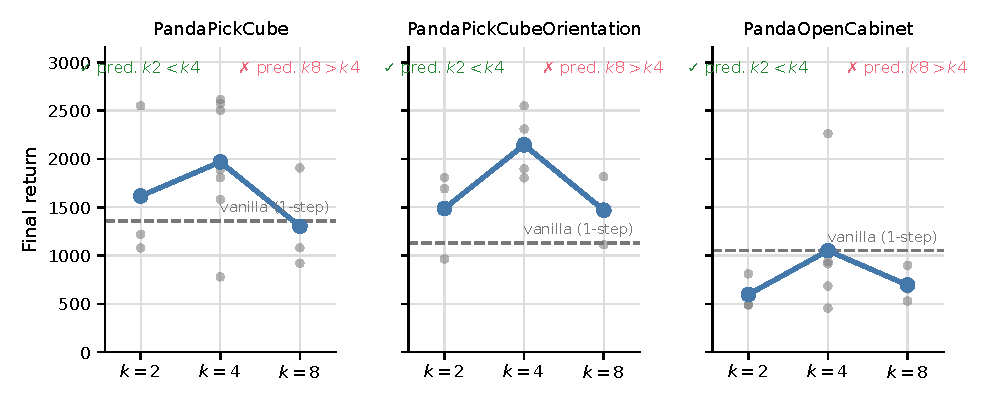
\includegraphics[width=\linewidth]{figures/fig_ksweep.pdf}
\caption{\textbf{The temporal-abstraction $k$-sweep behind the 4/4-vs-0/3 score.} Final return of the jumpy $k$-step world model at $k \in \{2,4,8\}$ on the three manipulation tasks (blue line: mean; gray dots: individual seeds; dashed gray line: mean of the matched vanilla 1-step baseline). New cells ($k{=}2$, $k{=}8$) are $n{=}3$ seeds each; the $k{=}4$ anchors are $n{=}8$ (PandaPickCube) and $n{=}5$ (Orientation, OpenCabinet); vanilla baselines $n{=}8/5/5$. Pre-registered, committed-before-harvest predictions from \texttt{disc\_err\_gap} scored \checkmark\ on every $k{=}2$ comparison (plus the cross-task gain ordering, 4/4 total) and $\times$ on every $k{=}8$ comparison (0/3) --- and the dose--response is unimodal with $k{=}4$ optimal on all three tasks. Data: \texttt{evidence/p1\_ksweep\_harvest.json}, \texttt{evidence/p1\_score.json}, \texttt{evidence/anchor\_jumpy\_vs\_vanilla.json}.}
\label{fig:ksweep}
\end{figure}

\textbf{4/4 on the $k{=}2$ block; 0/3 on the $k{=}8$ block (Figure~\ref{fig:ksweep}).} The honest reading: \texttt{disc\_err\_gap} is a real \emph{cross-task} predictor at fixed $k$ (7/7 ordering facts across two $k$ values) but it is \textbf{not $k$-invariant} --- iterating the 1-step model $k$ times inflates disagreement mechanically with $k$, so \emph{upward} cross-$k$ comparisons are confounded; the committed $k{=}8$ predictions walked into that confound and died in public, exactly as pre-registration is supposed to work.\footnote{Evidence file: \texttt{evidence/p1\_score.json} (\texttt{summary.interpretation}) in the paper repository.} A bonus result from the same harvest: the dose--response is \textbf{unimodal, with $k{=}4$ optimal on all three tasks} (Pick $1969 > 1616 > 1302$; Ori $2145 > 1487 \approx 1469$; Cab $1050 > 694 > 596$ for $k{=}4$ / $k{=}2$ / $k{=}8$ respectively) --- temporal abstraction has an optimal grain, neither too fine nor too coarse.\footnote{Evidence files: \texttt{evidence/p1\_score.json}, \texttt{evidence/p1\_ksweep\_harvest.json} in the paper repository.}

\subsection{Mechanism-check asymmetry: NO-GOs kill reliably, GOs only license}
\label{sec:goasym}

The same week produced two further mechanism-checks, and with them a finding about the method itself. The first, on a Hermite-spline action bottleneck (macro-action $=$ spline knots, shrinking the planner's search dimension), died at its pre-registered gate: open-loop spline replay at knot spacing 4 preserved a mean \textbf{0.364} of expert return against a 0.95 gate (zero-order hold: 0.305) --- one dev-box run instead of a 30-run fan-out.\footnote{Evidence file: \texttt{evidence/spline\_mechcheck\_PandaPickCube.json} in the paper repository. Stated caveat in the evidence file: the replay is open-loop while the reference rollout is closed-loop, so a marginal fail would not be fatal; 0.364 vs 0.95 is not marginal.}

The second is the instructive one. A macro-$Q$ error decomposition for a \emph{value-equivalent macro head} (pre-registered gates: GO iff value-cost ratio $\geq 0.3$ and Spearman $\rho \geq 0.4$) said \textbf{GO on Orientation} (value-cost ratio 0.352, $\rho = 0.57$ --- the macro-model's latent errors systematically cost value) and \textbf{NO-GO on OpenCabinet} ($\rho = 0.23$ --- errors large but value-unstructured).\footnote{Evidence files: \texttt{evidence/p3\_macroq\_ori.json}, \texttt{evidence/p3\_macroq\_cab.json} in the paper repository.} Yet the archive already contained the experiment: a value-equivalence loss on the macro head scored a final return of \textbf{583} ($n{=}3$) versus jumpy's 2145 ($n{=}5$) on Orientation --- catastrophic harm on exactly the task the mechanism-check green-lit.\footnote{Source repository: \texttt{docs/CHANGELOG.md} (2026-06-12 entry); per-seed finals 431/732/585 read from the \texttt{phasei27\_ve} PandaPickCubeOrientation worker CSVs (mean of MPPI evaluations from step 400k), mirrored in the source repository.} The asymmetry we record: \textbf{mechanism-check NO-GOs kill reliably; GOs license a test but never predict success.} This is consistent with the redundancy criterion's own logic --- C1/C2 are headroom (NO-GO-shaped) instruments: they can certify that an objective has nothing to gain, but passing them establishes only that a gain is not excluded.

\section{Limitations}
\label{sec:limitations}

We are deliberately conservative about scope.

\begin{itemize}
\item \textbf{Value-decodability was never validly measured --- in-distribution or out.} The linear value-decode probe is retracted as an instrument (Section~\ref{sec:monolithic}, Figure~\ref{fig:r2disc}): its high readings ($R^2=0.9994$ on the on-policy state distribution of a trained checkpoint\footnote{Evidence file: \texttt{evidence/value\_probe\_selfpred\_pick\_n12.json} in the paper repository.}) are saturated by construction and certify nothing --- in particular they do \textbf{not} certify that value stays decodable out-of-distribution or at held-out compositional counts. The criterion's own predictive direction (Section~\ref{sec:predictions}) hinges on exactly that OOD question, and a valid OOD measurement first requires a probe that discriminates in-distribution, which we do not yet have. This is the single most important caveat and the one the literature survey flags explicitly.\footnote{Source repository: \texttt{docs/research/graph-wm-dr/dr1-fable5-graph-wm-se-survey.md}, ``Caveats''.}

\item \textbf{Small world-model scale.} The transformer-WM NO-GO is on a $\sim$16k-step checkpoint;\footnote{Evidence file: \texttt{evidence/se\_attn\_trained.json} (meta block) in the paper repository.} the dreamer-family transformer training loop was dispatch-bound ($\approx$1\% GPU utilization), capping how far we could train before measuring.\footnote{Source repository: \texttt{docs/iterations/iteration\_28\_plan.md}, ``DREAMER4 / transformer-WM PERF BLOCKER''.} A better-trained / larger transformer-WM could in principle develop attention structure absent here; the NO-GO is for this scale.

\item \textbf{Single-object manipulation.} The monolithic and token-transformer classes are measured on single-object Franka tasks (and a single-agent CheetahRun for the SimNorm SE gap). Genuinely relational domains (multi-object, multi-agent) are exactly where the entity-graph class might break C1 OOD --- untested here at full scale on \emph{real} tasks; in the synthetic world the hardened sweep (Section~\ref{sec:entitygraph}, $n{=}4$, $N' \le 14$) finds no re-fit decodability collapse and no entity-graph advantage, leaving only the real-task cell open.

\item \textbf{The entity-graph data point is synthetic and single-seed.} The value-coupling NO-GO of Section~\ref{sec:entitygraph} is on a small entity-transformer WM in a synthetic world, at one seed, under the input-cross-Hessian operationalization; the message-level / attention-edge-ablation operationalization is untested, and the OOD-by-distractor variant is confounded by identity embeddings.\footnote{Evidence file: \texttt{evidence/gate0b\_vcoupling.json} in the paper repository.}

\item \textbf{Seed counts are modest.} The jumpy anchor is $n{=}5$ per arm with persisted CIs ($n{=}8$ on PandaPickCube after the boost);\footnote{Evidence files: \texttt{evidence/anchor\_jumpy\_vs\_vanilla.json}, \texttt{evidence/p1\_score.json} (\texttt{pick\_anchor\_n8}) in the paper repository.} 2 of 3 tasks are CI-separated (PickCube at $n{=}8$, Orientation at $n{=}5$), the third is null. Several ledger nulls are decisive in \emph{direction} at small $n$ but not all reach the full $n{=}5$ CI gate.\footnote{Source repository: \texttt{docs/iterations/RESEARCH\_LEDGER.md}.}

\item \textbf{The scored predictor (Section~\ref{sec:scored}) has its own caveats.} Each new $k$-sweep cell is $n{=}3$ seeds (only the $k{=}4$ anchor arms have $n{=}5$--$8$); the \texttt{disc\_err\_gap} reference values were computed from a \emph{single} checkpoint per task at $k{=}4$, so seed-robustness of the signal itself is unverified;\footnote{Evidence files: \texttt{evidence/p1\_ksweep\_harvest.json} (per-seed finals), \texttt{evidence/p1\_temporal\_signals.json} ($n{=}1$ checkpoint per task at $k{=}4$) in the paper repository.} and the mechanical-inflation confound that explains the $k{=}8$ failure was identified \emph{post hoc} --- the prediction failure itself was pre-registered, the explanation was not. A cross-domain out-of-sample test (CheetahRun, predicted ``weak-positive'' from gap 1.017 in the pre-registered ambiguous zone) is committed and pending; its outcome is deliberately \textbf{not} included here.\footnote{Evidence file: \texttt{evidence/p1\_ksweep\_prediction.json} (\texttt{pre\_registered\_prediction\_cheetah}) in the paper repository.}
\end{itemize}

Every quantitative claim in this paper is backed by a persisted JSON in the \texttt{evidence/} directory of the paper repository (the retracted value-probe readings, retained as documentation of the failed instrument --- $R^2=0.9994$ and the ve-checkpoint re-runs 0.9728/0.9505/0.9773 at $R^2=0.9998$--$1.0$ --- together with the discrimination experiment that retired them; attention-graph NO-GO gaps; SimNorm SE gap 53.1\%/47.2\%; jumpy anchor aggregation with $n{=}5$ CIs plus the $n{=}8$ PickCube resolution; synthetic value-coupling gate; the $k$-sweep prediction/score/harvest files and the spline and macro-$Q$ mechanism-checks) --- with the single exception of the archival 583-vs-2145 value-equivalence final, which is read from the source repository's mirrored worker CSVs and changelog as footnoted in Section~\ref{sec:goasym}.

\section{Related work}
\label{sec:related}

\paragraph{Structured / object-centric world models.} The control track record of structured WMs is mixed: DLPWM underperforms DreamerV3 \citep{ferraro2025dlpwm,hafner2025dreamerv3}; DreamerV3 beats its SLATE-slot variant \citep[ROCA;][]{ugadiarov2023roca}; ObjectZero $\approx$ EZ-V2 \citep{vakhitov2026objectzero}; the clearest win \citep[SOLD;][]{mosbach2024sold} is on bespoke relational manipulation with few seeds and is not replicated; token-transformer WMs \citep[IRIS, STORM;][]{micheli2023iris,zhang2023storm} are competitive but monolithic-token.\footnote{Source repository: \texttt{docs/research/graph-wm-dr/dr1-fable5-graph-wm-se-survey.md}, ``Comparison'' tables.} The consistent reading is that structure helps prediction and interpretability, not in-distribution control --- which the redundancy criterion explains as C1+C2 holding for strong monolithic latents. Recent reconstruction-free WMs continue to propose new \emph{representation} objectives --- e.g.\ R2-Dreamer's Barlow-Twins-style redundancy-reduction loss, competitive with DreamerV3 and TD-MPC2 without a decoder \citep{morihira2026r2dreamer} --- but these \emph{replace} the backbone's representation objective rather than adjoin an explicit abstraction to an already-strong self-predictive latent, and their reported gains concentrate where the reconstruction objective demonstrably fails (tiny task-relevant objects), consistent with our reading that headroom exists only where the backbone objective leaves value-relevant structure unextracted.

\paragraph{Structural entropy in RL.} SE \citep{li2016structural} has been used for state/action/skill abstraction on precomputed transition or value graphs via discrete greedy encoding-tree minimization \citep[SISA, SIDM, SIRD, SI2E;][]{zeng2023sisa,zeng2024sidm,zeng2024si2e}, and differentiable SE exists for static graph clustering \citep[LSEnet, DeSE;][]{sun2024lsenet} --- but a differentiable SE loss \emph{inside} a WM latent is an empty gap.\footnote{Source repository: \texttt{docs/research/graph-wm-dr/dr1-fable5-graph-wm-se-survey.md}, ``Comparison: SE methods''.} Our contribution is to show, with cheap mechanism-checks, that this gap is most likely null-shaped on current monolithic and token-transformer substrates, and to specify the one substrate (value-coupled entity graphs, OOD) where it might not be.

\paragraph{Self-predictive and value-equivalent abstraction.} \citet{ni2024bridging} on self-predictive sufficiency and \citet{grimm2020value} on value equivalence provide the theory that condition (1) operationalizes; the criterion is, in effect, an empirically-measurable test of when those theories' ``sufficient abstraction'' has already been attained by a self-predictive backbone. The bisimulation line remains active on exactly our substrate family, with published positive results we do not replicate: BS-MPC \citep{shimizu2025bsmpc} adds a bisimulation-metric loss to the TD-MPC encoder and reports stability and noise-robustness gains on DMC, and \citet{toso2026invariant} add a bisimulation encoder to a joint-embedding predictive WM (DINO-WM-style, pretrained visual features) and report robustness gains under visual distractors. Our single-variable replication of a BS-MPC-style auxiliary on TD-MPC2's SimNorm latent was actively harmful (Table~\ref{tab:nulls}, \#3), and the distractor-robustness-from-abstraction lever was falsified on our substrate (\#4); the reconciliation we find most plausible --- and cannot rule out otherwise --- is that the reported gains live where the latent is \emph{not} already value-sufficient (pixel-based latents, frozen pretrained encoders, or the weaker TD-MPC1 backbone), which is precisely the headroom the criterion predicts, but this makes the substrate-dependence of bisimulation gains an explicit open question rather than a settled null.

\paragraph{Probing as representation evaluation.} \citet{zhang2024lightweight} propose light-weight linear probing --- of environment reward and expert actions --- as a cheap proxy for the quality of \emph{frozen, unsupervised-pretrained} representations, and find it rank-correlates with downstream RL performance on Atari100k. Our discrimination result (Section~\ref{sec:monolithic}, Figure~\ref{fig:r2disc}) does not contradict this but narrows its scope: probe validity is operationalization-dependent. Probing the agent's \emph{own} value head against its \emph{own} co-trained latent is saturated by construction, and probing Monte-Carlo returns is confounded by policy-dependent return variance --- so a probe with an exogenous target compared \emph{across} fixed encoders can rank representations even though the same instrument cannot certify value-sufficiency of a single latent co-trained with its value function.

\paragraph{Methodology.} The campaign's transferable by-product is the protocol itself --- single-variable, compute-matched, peak-and-final pre-registered CI gates \citep{agarwal2021rliable}, mechanism-check before fan-out --- which caught 8 mirages and killed SE-flavored levers in an afternoon rather than a multi-week build.\footnote{Source repository: \texttt{docs/iterations/RESEARCH\_LEDGER.md}, ``WHAT WORKED''.}

\section{Conclusion}
\label{sec:conclusion}

We converted a 16-lever campaign of null explicit-abstraction results into a single falsifiable predictive criterion: explicit abstraction is redundant for a world model exactly when its latent is (1) linearly value-decodable and (2) its interaction graph already carries task-aligned structure. For the monolithic SimNorm class we measured C2 directly (a 53.1\% SE transition-graph gap that is real but motion-phase / control-irrelevant) and found C1 to be \emph{unmeasurable by its own probe} --- the seemingly decisive $R^2=0.9994$ reading is saturated by construction and was retracted --- so redundancy for this class is established not by the probe but by the direct record: the campaign's nulls and a matched, multi-seed 16-task DMC benchmark on which the structural-entropy abstraction ties the monolith on return while costing $\sim$1.35$\times$ wall-clock. We measured a clean C2 NO-GO for the token-transformer class (attention-graph SE gap at/below a degree-preserving null, trained $\approx$ untrained), and measured a synthetic instrument-validation NO-GO for the entity-graph class --- the last and most relational --- (the value-coupling cross-Hessian graph reads at chance, AP $=0.500$ / $z=-0.08$, despite a near-perfect reward fit and ground-truth coupling known by construction --- with the stated caveats), while the exact full-scale OOD value-decodability probe that would confirm or break the criterion on real multi-object tasks remains open. We give the null a mechanism: explicit abstraction is a \emph{basis change, not a capacity change} (Proposition~\ref{prop:dpi}); it cannot add task-relevant information to an already value-sufficient latent, and the benchmark's cost-without-return is the behavioral fingerprint of that relocation. On the converse, positive direction we scored a pre-registered predictor of where \emph{temporal} abstraction pays: \texttt{disc\_err\_gap} went 4/4 on its committed $k{=}2$ predictions and 0/3 at $k{=}8$ --- a real cross-task predictor at fixed $k$ whose $k$-invariance is falsified --- and the week's mechanism-checks crystallized an asymmetry worth stating: NO-GOs kill reliably, GOs only license a test. The criterion's value is that it is cheap to evaluate on any trained checkpoint and tells you, before a multi-week build, whether an abstraction objective has headroom --- and where to look (a latent that is \emph{not} value-decodable OOD) if you want to find a genuine positive case.

\bibliography{references}
\bibliographystyle{tmlr}

\end{document}
